%
% Copyright 2018 Markus Borg, Lund University
%
% This work is licensed under a Creative Commons Attribution-ShareAlike 4.0 International License.
% See http://creativecommons.org/licenses/by-sa/4.0/
%
% The dodument is based on a LaTeX template developed by Jean-Philippe Eisenbarth
% https://github.com/jpeisenbarth/SRS-Tex
%
\documentclass{scrreprt}
\usepackage{graphicx}
\usepackage{listings}
\usepackage{underscore}
\usepackage[bookmarks=true]{hyperref}
\usepackage[utf8]{inputenc}
%\usepackage[english]{babel}
\hypersetup{
    bookmarks=false,    % show bookmarks bar?
    pdftitle={Lab 4},    % title
    pdfauthor={Markus Borg},                     % author
    pdfsubject={TeX and LaTeX},                        % subject of the document
    pdfkeywords={TeX, LaTeX, graphics, images}, % list of keywords
    colorlinks=true,       % false: boxed links; true: colored links
    linkcolor=blue,       % color of internal links
    citecolor=black,       % color of links to bibliography
    filecolor=black,        % color of file links
    urlcolor=purple,        % color of external links
    linktoc=page            % only page is linked
}%
\def\myversion{0.2 }
\date{}
%\title
\usepackage{hyperref}
\begin{document}

\begin{flushright}
    \rule{16cm}{5pt}\vskip1cm
    \begin{bfseries}
    	\LARGE{ETSA02-ADM-LAB4}\\
    	\vspace{1.5cm}
        \Huge{Lab 3}\\
        \vspace{0.5cm}
        Code coverage testing\\
        \vspace{0.5cm}
        and static code anaysis\\
        \vspace{1.5cm}
        \LARGE{Version \myversion approved}\\
        \vspace{1.5cm}
        Prepared by Markus Borg\\
        %\vspace{1.5cm}
        Dept. of Computer Science, Lund University\\
        \vspace{1.5cm}
        \today\\
    \end{bfseries}
\end{flushright}

%\tableofcontents

\chapter*{Revision History}

\begin{center}
    \begin{tabular}{|c|c|c|c|}
        \hline
	    Name & Date & Reason For Changes & Version\\
        \hline
	    Markus Borg & 2018-04-18 & Initial structure. & 0.1\\
        \hline
        Markus Borg & 2018-04-21 & Added EclEmma, SpotBugs, and SonarLint. & 0.2\\
        \hline
    \end{tabular}
\end{center}

\chapter{Introduction}
Lab 4 focuses on source code quality assurance for Basic Melee Bot. High-quality source code is your best approach to decrease the chances of releasing a robot with bugs, and it also greatly improves the maintainability of the product. First, you will add code coverage measurements to your existing suite of unit tests. Second, you will explore two established tools for static code analysis. Finally, you will generate Javadoc for Basic Melee Bot, i.e., the de facto industry standard for documenting Java classes. More specifically, Lab 4 covers the following:

\begin{itemize}
\item Code coverage testing with EclEmma
\item Static code analysis with SpotBugs and SonarLint
\item Generating Javadoc from Eclipse
\end{itemize}

\chapter{Before the lab}
If you still have the Java project from either Lab 2 or Lab 3 in your workspace, then you have everything you need for Lab 4. The source code used in Lab 4 is Basic Melee Bot and its accompanying unit test suite (introduced in Lab 2, but available also in Lab 3). On the other hand, if you are now comfortable with downloading and importing source code from GitHub, you can of course download the latest version. If you want the latest code, Lab 4 has been prepared in the course repository on GitHub:\\https://github.com/lunduniversity/introsofteng\\\\
The same instructions as from Lab 2 and Lab3 apply: if you have already cloned the repository, pull the latest source code to make sure you work with the latest version. If you prefer downloading the code, instead click the button presented in Figure~\ref{fig:github} and choose ``Download ZIP''. Once downloaded, locate the files you need for Lab 4. The files are in the folder introsofteng-master/labs/lab4/src, and its subfolder: `test'. Rewatch the video ``Lab2_download.avi'' on Google Drive (ETSA02 Everyone/Labs) if you need support.

To prepare for the lab session, please make sure you can execute a unit test suite for Basic Melee Bot. Then have a look at the following pages:
\begin{itemize}
\item Code coverage (skip ``Modified condition/decision coverage'' and onwards)\\-- https://en.wikipedia.org/wiki/Code_coverage
\item EclEmma homepage (browse the page to get a high-level understanding) \\-- http://www.eclemma.org/
\item Coverage counters in JaCoCo (library used by eclEmma) \\-- hhttp://www.eclemma.org/jacoco/trunk/doc/counters.html
\item Static code analysis (skip ``Formal methods'') \\-- https://en.wikipedia.org/wiki/Static_program_analysis
\item SpotBugs homepage (browse the page to get a high-level understanding) \\-- https://spotbugs.github.io/
\item SonarLint homepage (browse the page to get a high-level understanding) \\-- https://www.sonarlint.org/
\item Javadoc document generator \\-- https://en.wikipedia.org/wiki/Javadoc
\end{itemize}

\chapter{At the lab} \label{sec:atlab}
In Lab 4, you will learn to download open source tools from the big Eclipse ecosystem through Eclipse Marketplace. You reach Eclipse Marketplace directly from your Eclipse installation: Select ``Eclipse Marketplace...'' from the Help menu.

\section{Code coverage with EclEmma}
First, you will work with code coverage testing. Search for EclEmma on Eclipse Marketplace, and install the latest version: EclEmma Java Code Coverage 3.0.1. EclEmma introduces a new run option in Eclipse, beyond ``Run as...'' and ``Debug as...''. The new run option is called ``Coverage as...''. The eclEmma ``Coverage view'' automatically appears when a new coverage session is added or can manually be opened from the Window $\rightarrow$ Show View menu in the Java category. 

The coverage view shows code coverage summaries for the active session. Individual columns in the view contain the following numbers for the active session, always summarizing the child elements of the respective Java element:

\begin{itemize}
\item Coverage ratio
\item Items covered
\item Items not covered
\item Total items
\end{itemize}

The elements may be sorted in ascending or descending order by clicking the respective column header. Double-clicking an element opens its declaration in an editor with highlighted source code. Figure~\ref{fig:eclemma} shows an example of the coverage view, and how to switch between different coverage metrics, i.e., instruction counters, branch counters, line counters, method counters, type counters, and complexity.  

\begin{figure}
\centering
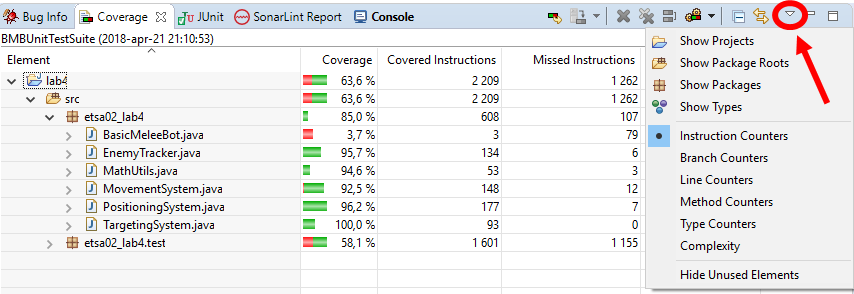
\includegraphics[width=0.99\textwidth]{figures/EclEmma.png}
\caption{The coverage view in EclEmma. The circle shows where to switch coverage metric.}
\label{fig:eclemma}
\end{figure}

Time to perform a code coverage measurement of Basic Melee Bot to analyze to what extent the unit test suite covers the source code of the robot. In the ``Package Explorer'' in Eclipse, right click the unit test suite in your Java project (``AllBasicMeleeBotUnitTests.java'' if working with Lab 2, otherwise ``BMBUnitTestSuite.java'') and choose ``Coverage as'' $\rightarrow$ JUnit Test. The unit test suite will run as before, but you will also get coverage measurements. Explore the results in the EclEmma coverage view (skip coverage of the classes in the test package). Double click on elements in the coverage view to navigate to color coded source code, for which green = covered, yellow = partly covered, and red = not covered. Then try to answer the following questions:
\begin{itemize}
\item What is the total instruction coverage?
\item Which classes have the highest instruction coverage? Why?
\item Which classes have the lowest instruction coverage? Why?
\item What do the other coverage metrics reveal?   
\end{itemize}

\chapter{After the lab}
Your group shall state a code coverage target for your unit test suite in the STS, at least instruction coverage. For the Final Release of your robot, you shall measure code coverage using EclEmma and report the outcome in the test report. Any deviations from the coverage target shall be motivated.




\end{document}
